\documentclass[11pt,dvipdfmx]{article}


\usepackage{deauthor,times,graphicx}
\usepackage{booktabs} 
\usepackage{amsmath}
\usepackage{epstopdf}
\usepackage{verbatimbox}
\usepackage{multirow} 

%\graphicspath{{athanassoulis/}}


\newcommand\Paragraph[1]{\vspace{0.02in}  \noindent \textbf{#1.}}
\newcommand\Paragraphqit[1]{\vspace{0.02in}  \noindent \textit{#1?}}
\newcommand\Paragraphbit[1]{\vspace{0.02in}  \noindent \textbf{\textit{#1.}}}

\begin{document}



\title{Building Deletion-Compliant Data Systems}


\author{
Manos Athanassoulis, Subhadeep Sarkar, Tarikul Islam Papon, Zichen Zhu, Dimitris Staratzis
\medskip\\
Boston University
}



\maketitle


\begin{abstract}
Most modern data systems have been designed with two goals in mind -- fast ingestion and 
low-latency query processing. The first goal has led to the development of a plethora of 
write-optimized data stores that employ the \textit{out-of-place} paradigm. 
Due to their write-optimized design, out-of-place data systems perform deletes 
\textit{logically} via invalidation, and retain the invalid data for arbitrarily long. 
However, due to the recent enactment of new data privacy regulations, 
the requirement of \textit{timely deletion of user data} has become central. 
% One primary focus of privacy regulations is to establish the user's 
The \textit{right to be 
forgotten} (in EU's GDPR), \textit{right to delete} (in California's CCPA and CPRA), or 
\textit{deletion right} (in Virginia's VCDPA) mandates that service providers persistently delete a user's data within a pre-set time duration. 
Logical deletion in out-of-place data systems, however, does not offer guarantees for 
\textit{timely and persistent deletion}, and attempting to enforce it using existing tools 
leads to poor performance and increased operational costs. 

\hspace{0.02in} In this paper, we present a new framework for building \textit{deletion-compliant
data systems} from a holistic perspective. We analyze the new regulations and the 
requirements derived from the new policies, and we propose changes in the application and
the system layer of data management. We outline the new types of deletion requests that need to be supported, the query language
modifications needed to be able to request for timely persistent data deletion, and the system-level 
changes needed to realize timely and persistent deletes. 
The proposed framework for deletion compliance lays the groundwork for a new class of data 
systems that can offer system-level guarantees for user data privacy. We present recent results 
spanning all layers of the framework: the requirements and
the application layer target any database system, while the system layer discussion is geared 
towards out-of-place systems. Finally, we conclude with a discussion on next steps
and open challenges on building deletion-compliant data systems.

\end{abstract}





\section{Introduction}
\label{sec:introduction}


Data-intensive social and commercial applications and new advancements in domains like Internet-of-things, edge computing, 5G communications, and autonomous vehicles, generate a vast amount of \textit{personal data} processed by several data companies~\cite{Cisco2018,Gartner2017}. 
The increasing demand for efficient collection, storage, and processing of user data over the past two decades, has driven the development of data systems that can \textit{sustain high ingestion rates} without compromising the ability to \textit{access and analyze the data quickly}. 

\newpage
\Paragraph{Out-of-Place Systems}
The need for optimizing data ingestion while maintaining efficient data access has led
to the prominence of the \textit{out-of-place} paradigm, which fulfills these goals by
minimizing the interference between reads and writes. Today, several commercial relational and 
array-based data 
stores~\cite{Athanassoulis2011,Deng2020,Farber2012,Heman2010,Idreos2012,Kang2016,Lamb2012,Sadoghi2016,Stonebraker2005} and NoSQL data 
stores~\cite{ApacheAccumulo,ApacheCassandra,ApacheHBase,DeCandia2007,FacebookRocksDB,Golan-Gueta2015,Huang2019,Sears2012} have adopted the out-of-place paradigm. 

\textit{Relational and Array-based Systems}. 
Relational systems that buffer updates before applying them lazily on the base data, essentially, follow the out-of-place paradigm. 
The columnar and array data stores implemented by Vertica~\cite{Lamb2012,Stonebraker2005}, 
SciDB~\cite{Paradigm4,Stonebraker2013}, and TileDB~\cite{Papadopoulos2016,TileDB} use an in-memory storage component that stores incoming inserts, updates, and deletes out of place, and 
applies the changes lazily on the disk-resident data. Similarly, the state-of-the-art column-store system
MonetDB~\cite{Idreos2012} uses an in-memory positional index for incoming 
data~\cite{Heman2010}, and SAP HANA uses
a delta store per table to facilitate fast ingestion without affecting its 
read-optimized data layout~\cite{Farber2012}. 
Finally, several research-prototype systems
use a separate delta store on faster storage (e.g., SSDs/NVM) to 
offer efficient access to incoming 
data \cite{Athanassoulis2011,Athanassoulis2015,Deng2020,Kang2016,Sadoghi2016}.

\textit{NoSQL Systems}.
More than relational systems, production-grade NoSQL key-value stores predominantly employ the 
out-of-place paradigm, frequently based on the log-structured merge (LSM) paradigm.
An LSM-tree is a heavily write-optimized out-of-place data structure that maintains several on-disk components, which can be viewed as several out-of-place delta stores~\cite{ONeil1996,Dayan2017,Idreos2019,Luo2020b,Sarkar2022b,Zheng2018}.
Key-value stores such as RocksDB~\cite{Dong2017,FacebookRocksDB} and  LevelDB~\cite{GoogleLevelDB} at Facebook, BigTable~\cite{Chang2006} at Google, X-Engine~\cite{Huang2019,Yang2020} at Alibaba, Voldemort~\cite{LinkedInVoldemort} at LinkedIn, DynamoDB~\cite{DeCandia2007} at Amazon, Cassandra~\cite{ApacheCassandra}, HBase~\cite{ApacheHBase}, and Accumulo~\cite{ApacheAccumulo} at Apache, and bLSM~\cite{Sears2012} and cLSM~\cite{Golan-Gueta2015} at Yahoo are based on the log-structured merge (LSM) paradigm. 
Other out-of-place architectures employed by NoSQL systems are B$^+$-tree, B$^\epsilon$-tree, and fractal tree-based storage engines with \emph{buffering support}, such as COLA~\cite{Bender2000}, TokuDB~\cite{Kuszmaul2014}, and 
B\textit{e}rtFS~\cite{Bender2015,Jannen2015}. 

\textit{Cloud-based Systems}.
Cloud-based systems naturally employ the out-of-place paradigm as they rely on the 
immutability of cloud storage. Hence, systems like Amazon 
Redshift~\cite{AmazonRedshift,Gupta2015}, Cloud Data Platform~\cite{Dageville2016} at 
Snowflake, and Delta Lake~\cite{Databricks,Databricks2021} at Databricks employ variations
of the out-of-place paradigm in the interest of performance. 
Deletes and updates are initially performed logically and are gradually propagated to 
persistent media through periodic merging with base data. 

\Paragraph{Deletes in Out-of-Place Systems}
A key property of out-of-place systems is that they treat deletes (and updates) similarly to 
inserts, i.e., instead of deleting (updating) entries in-place, they insert a new version of 
the entry to be deleted that \textit{logically invalidates} the target entries. 
These special entries that are responsible for logical deletes are termed \textit{delete 
markers}~\cite{Lamb2012} or \textit{tombstones}~\cite{Dong2017,Sarkar2020}. 

Logical data deletion is a quintessential out-of-place operation, but it does not guarantee 
\emph{purging} of the data under deletion within a definite timeframe. Rather, the data is marked as
invalid; essentially, \emph{not accessible} to external users. In practice, logically 
deleted entries are kept for arbitrarily long in the system, since the time to definitively 
delete the data (termed \emph{persistent deletion}) depends on the state of the system, 
and not on when the user request expects the data to be deleted~\cite{Sarkar2020}.
In fact, most out-of-place data stores are built with the underlying assumption of 
\textit{perpetual data retention} in order to gain more insights from the user and 
organizational data~\cite{Whittaker2019}, hence \emph{timely persistent deletion} has not
been part of their design goals. In addition to deletes, logical updates in out-of-place 
systems are applied lazily too, however, the implications of out-of-place deletes are 
critical in terms of the privacy regulations, and thus, are our focus. 

\subsection{Problem: The Privacy Concern}
\Paragraph{Cost of Logical Deletes} Logical deletes and updates in out-of-place systems boost ingestion performance, however, they come at a significant cost.  
In fact, when tasked with deleting user data persistently in a timely manner, out-of-place systems suffer both in terms of (a) data privacy protection and (b) the overall system performance. 
Such systems are designed to retain the logically invalidated data indefinitely, and the time required for persistent removal of the physical data entries depends on (i) the data layout, (ii) the data re-organization policy (e.g., node splitting/merging in B-trees, compaction in LSM-trees, consolidation in TileDB), (iii) the design of the storage engine (such as the fanout of a tree and the size of a database), and (iv) the composition and distribution of the workload -- factors that are \textit{beyond the control of the application and system developers or administrators}. 
Thus, most out-of-place systems are unable to provide any latency guarantees for persistent deletion of user data~\cite{Sarkar2020}. 


\Paragraph{The Legal Frontier}
In recent years, a number of government-driven efforts across the globe unfolded, 
aiming to protect the privacy of user data and give back to the users the control of their 
personal data. On the legal side, regulations such as the EU's GDPR~\cite{GDPR}, California's 
CCPA~\cite{CCPA2018} and CPRA~\cite{CPRA}, and Virginia's 
VCDPA~\cite{VCPDA} have been introduced, which mandate that data companies ensure \textit{privacy through deletion}~\cite{Shastri2019,Shastri2021}. 
GDPR's \textit{right to be forgotten}, CCPA and CPRA's \textit{right to delete}, and the \textit{deletion right} in VCDPA particularly focus on \textit{persistent deletion of user data on-demand and in a timely manner}~\cite{Ambrose2013,Deshpande2018,Goddard2017,Jones2012,Sarkar2018,Shastri2019,Schwarzkopf2019,Tsesis2014}. 

\Paragraph{The Technological Roadblock} Treating \emph{deletes} as \textit{first-class citizens} is new for the data systems community, and it would require a significant amount of work to transform classical systems to be efficient deletion-wise. 
Even today, it continues to be a critical technological challenge for the biggest of data companies using state-of-the-art storage engines to demonstrate compliance with the deletion regulations and to efficiently delete user data on-demand~\cite{Shah2019,Shastri2020,Shastri2021}. 
To translate this into numbers, between January 2020 and January 2022, the penalties under GDPR paid by data companies amounted to more than \$1B, which includes large contributions from companies such as Amazon (\$877M), WhatsApp (\$255M), Google Ireland (\$102M), and Facebook (\$68M), H\&M (\$41M), British Airways (\$26M), and Marriot (\$23M)~\cite{Piper2022,DLAPiper2020,Tessian2022}. 
Thus, to demonstrate compliance, many companies end up performing expensive database-wide consolidations periodically (e.g., every few weeks), to ensure timely persistent deletion of user data~\cite{Sarkar2020,Sarkar2021c}. 
Such operations are remarkably expensive in terms of time and money, cause undesirable latency spikes, and hence, should be avoided. 

\begin{figure*}[tb]
    \centering
        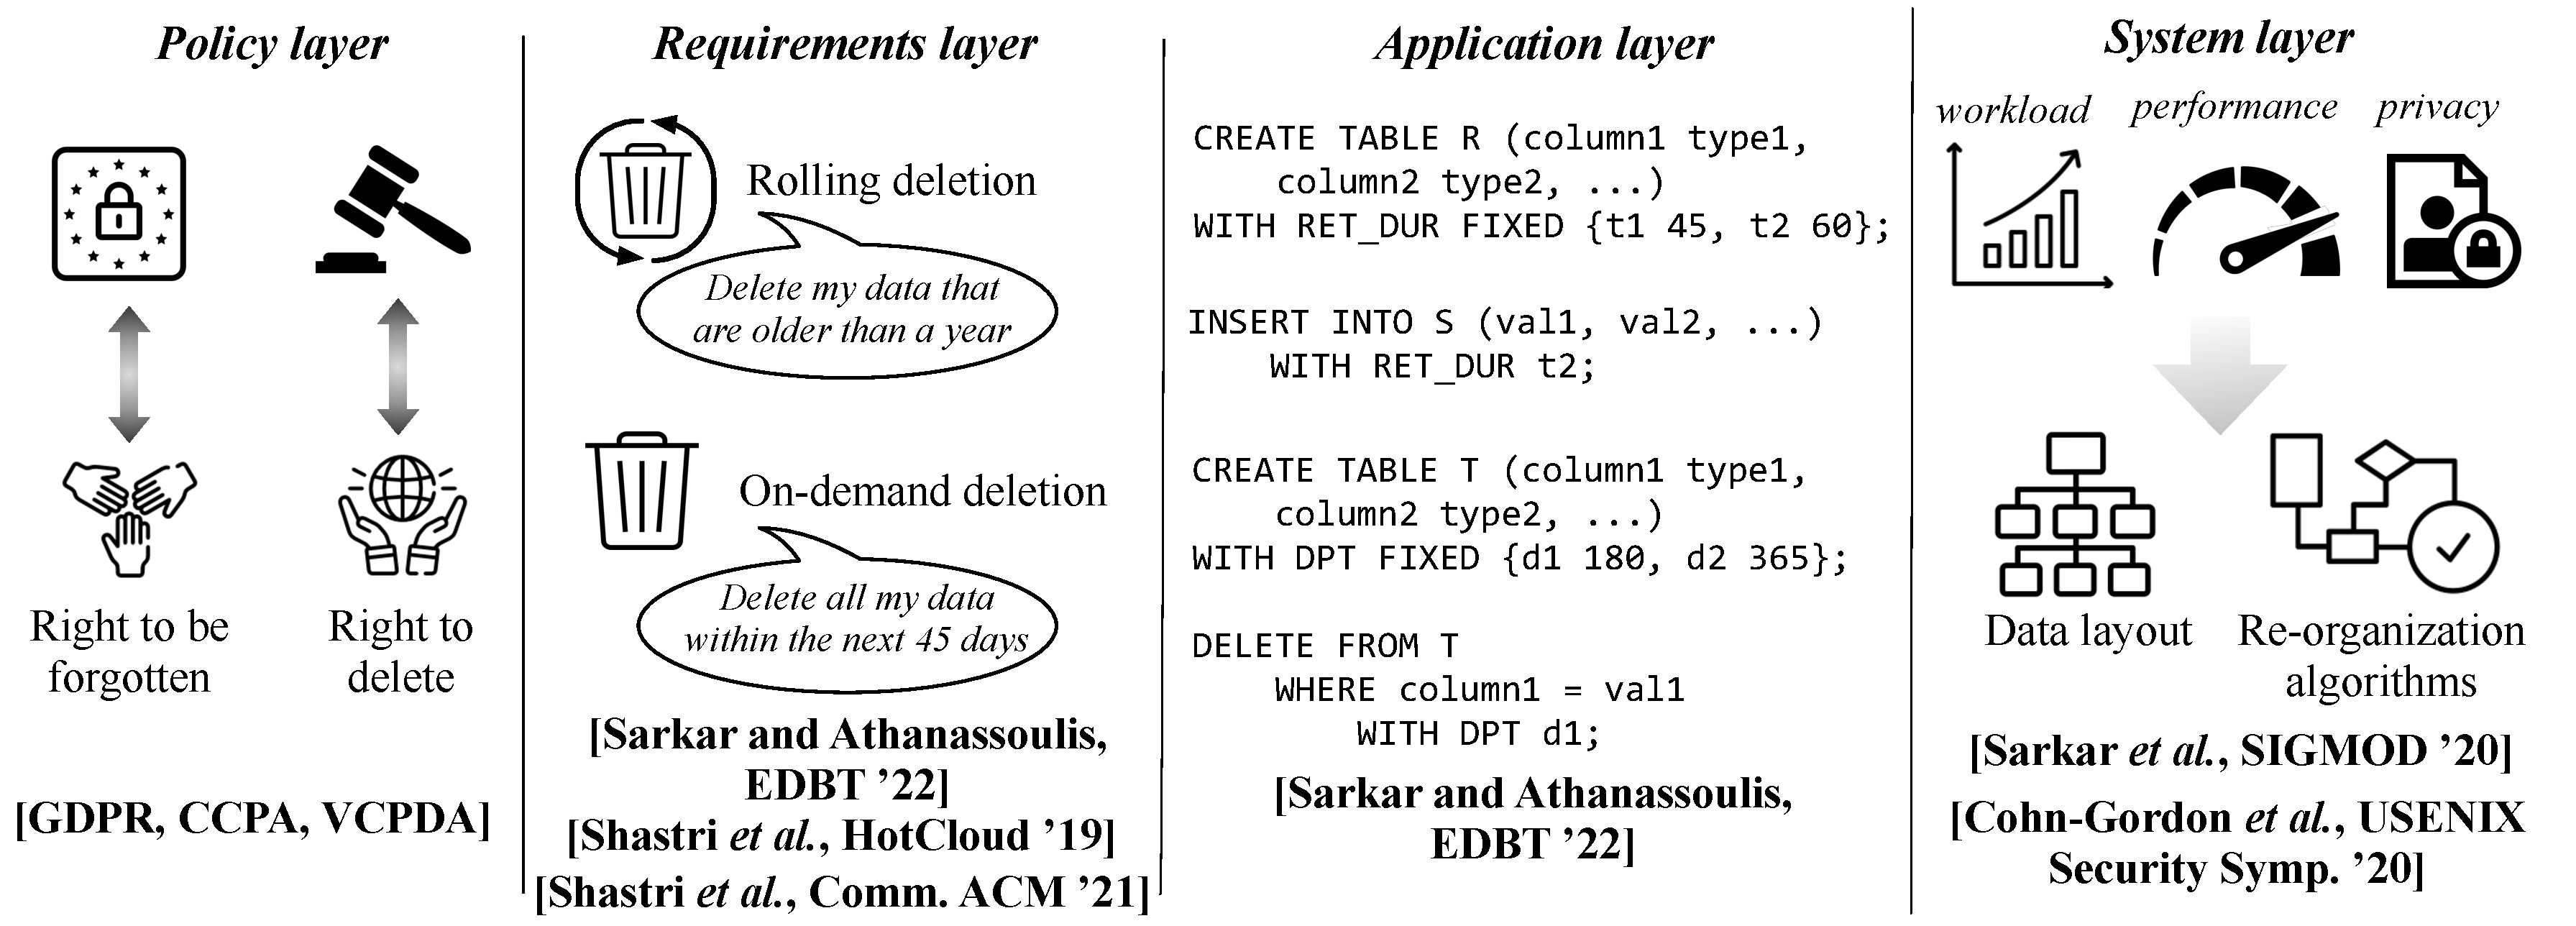
\includegraphics[scale=0.29]{figs/layered_problem_scenario.pdf}
    \vspace{-0.25in} 
    \caption{The four layers of deletion-compliant data systems.}
     \vspace{-0.1in}
    \label{fig: vision}
\end{figure*}

 
\subsection{Deletion-Compliant Data Systems}
In this paper, we present our vision and first results on designing data systems that ensure data privacy through timely and persistent deletion of user data. 
Existing efforts that attempt to delete user/application data on-demand suffer in terms of performance as the underlying data layout and data management mechanisms are ill-suited for the purpose. 
We identify the missing links, in terms of technological tools, both at the application level and the system level, and we propose a hierarchical framework that enables our vision of privacy through deletion in out-of-place data systems (Figure~\ref{fig: vision}).



\newpage
\Paragraph{Roadmap} 
The privacy through deletion framework is a roadmap toward building deletion-compliant data systems. 
We begin by outlining the challenges associated with each layer of our vision, i.e., in the context of (i)~translating the legal mandates to user requirements, (ii) expressing the user requirements through a declarative API, and (iii) realizing the application-level requirements at the system level.
Next, we identify and categorize the different classes of user requests for deletes in light of the legal regulations. 
Based on this, we present the challenges associated with transforming the classes of deletion requests into application-level specifications, and we propose an SQL extension as an example that can be extended to other query languages to support deletion of user data \textit{periodically} and \textit{on-demand}. 
Further, we outline the design and tools necessary at the system level to support the application-level requirements. 
Finally, we conclude with a discussion on how the proposed framework drives us toward building deletion-compliant data systems, and what further research challenges remain open to fully realize this vision.






%
 
\section{From Regulation to Practice}
\label{sec:legal}


The legal landscape for data privacy has changed drastically over the past few years, and governments across countries, as well as across different states in the US, have enforced acts and regulations to control the consumption of user data by service providers and give back to the users the control of their personal data. 
Translating the new regulations to new \emph{user-data privacy-compliant system behavior}
still faces significant challenges. In this section, we present in more detail the 
requirements from the regulation point of view, and we showcase through three realistic
scenarios the limitations of the state-of-the-art data systems when tasked to implement
these requirements. 


\subsection{Regulations on Timely Data Deletion}
While the new regulations propose an array of new requirements, we particularly focus on the legal 
policies concerning data retention and data deletion, with the objective of ensuring 
\textit{privacy through deletion}. 

\Paragraph{Right to be Forgotten, \textit{EU GDPR}}
The General Data Protection Regulation (GDPR) has revolutionized the data privacy and security landscape across the European Union countries~\cite{GDPR}. 
One of the fundamental changes introduced through the GDPR (over the older Data Protection Act (DPA) that it replaced), is the \textit{right to be forgotten}, which empowers the users with the \emph{right} to request a service provider to delete all their personal data persistently from its domain. 
Such deletion requests may be presented either up-front or on-demand. 
The service provider must comply with those requests, unless it has compelling reasons for acting otherwise (Art. 17(3)). 


\Paragraph{Right to Delete, \textit{CCPA}, \textit{CPRA}}
The California Customer Protection Act (CCPA), which will eventually be replaced by the California Privacy Rights Act (CPRA) in 2023, allows the users/consumers in California to request from service providers to permanently delete all data personal to the user~\cite{CCPA2018,CPRA}. 
Under CCPA and CPRA, the service providers must acknowledge such a user request within $10$ days, and respond to the request within $45$ business days~\cite{Brown2021}. 
Persistent deletion must be performed by removing the target data across all domains, barring archive and backup systems, along with data anonymization as required. 

\Paragraph{Right to Delete, \textit{VCDPA}}
Similarly to CCPA, the Virginia Consumer Data Protection Act (VCDPA) empowers users in Virginia to exercise their right to delete their personal data from a provider's domain~\cite{VCPDA}. 
VCDPA requires the service providers to serve a delete-request from a user within $45$ business days~\cite{Brown2021}. 


\Paragraph{Right to be Forgotten, \textit{UK GDPR, DPA}} 
The UK GDPR, along with the Data Protection Act (DPA) 2018 provides the country's citizens with similar rights about personal data deletion as the EU GDPR. 
The users are allowed to express their deletion preference verbally or in writing, to which the service providers must respond within $30$ days~\cite{UKGDPR,DPA2018}. 



\Paragraph{Other Efforts}  
Among other countries, Argentina~\cite{Carter2013,Pardo2020}, Singapore~\cite{Chik2013}, India~\cite{Kittane2021}, Canada~\cite{PIPEDA2019}, and South Korea~\cite{Brown2016} have some implementation of the right to deletion as a part of their respective privacy protection acts.



\subsection{Limitations of the State of the Art} 
In light of the deletion regulations, we now present three real-life scenarios to highlight why state-of-the-art data systems are ill-equipped to support deletes efficiently without hurting performance. 
We do so by identifying the missing links in different hierarchical levels of the proposed privacy-through-deletion framework.
Below, we illustrate (i) that the users are unable to express their preferences about deleting their personal data, (ii) why it is difficult for application developers to support the deletion requests from the users, and (iii) why it is difficult to realize persistent deletes in a timely manner in live production servers.


\textit{Scenario 1}: \textit{Alice} is a user of a smart-home ecosystem, \textit{HomeComp}, which provides real-time services including video surveillance, remote temperature, and illumination control. 
\textit{Alice} enjoys the services of \textit{HomeComp}, but concerned about her personal data privacy, she wants \textit{HomeComp} to permanently delete all her data older than $30$ days on a rolling basis.  

\Paragraphqit{The problem}
Like most service providers, \textit{HomeComp}'s data model is built around the assumption of perpetual data retention; deletion of user data needs a human-in-the-loop that performs the necessary actions.
Thus, \textit{HomeComp} does not allow its user to request for rolling timestamp-based data deletion. 

\textit{Scenario 2}: \textit{StreamEra} is a company that provides real-time insights for data streams, and allows its users to request on-demand deletion of their personal data, as it is bound by the \emph{right to be forgotten}.
\textit{StreamEra} uses an SQL-based wrapper on top of its storage layer.

\Paragraphqit{The problem} 
While \textit{StreamEra} wants to serve its users by ensuring timely persistent deletion of their personal data, SQL does not provide support for such an operation.
Instead, the backend engineers implement the user-requested deletion functionality at the application level in an ad-hoc manner as it is not native to SQL.

\textit{Scenario 3}: A cloud-based online data analysis company \textit{ClouData}, stores user data using immutable files within its HTAP data store. 
\textit{ClouData} is bound by the \emph{right to be forgotten}, and thus, has to delete all user data that are older than $D$ days.

\Paragraphqit{The problem} As the data organization on disk is not based on the ingestion timestamp and aims to accelerate read queries, it uses the most frequently
queried attribute to partition. Hence, the objects qualifying for a timestamp-based
deletion may be dispersed within the data store. 
As in-place deletion is not supported due to immutability, state-of-the-art data stores periodically consolidate the entire data set to delete all invalid entries. 
Ensuring privacy via this approach is costly in terms of disk writes and overall accesses, and causes latency spikes leading to performance unpredictability. 

\Paragraph{Other Challenges of Logical Deletes} In addition to not complying with regulatory requirements, 
logical deletes may cause more hurdles. Specifically,
by retaining invalidated data (that should not be used anymore), a data company:

\begin{enumerate}
	\item Wastes storage space and energy on data that cannot exploit in any way. Further, data maintenance results in additional write amplification that wears off the underlying storage devices \cite{Athanassoulis2016}.
	\item Risks that a security leak will reveal user data that users expect to be deleted~\cite{Piper2022}.
	\item Hurts read performance, as its data management layer uses metadata and indexes for all data regardless of whether they are invalidated~\cite{Sarkar2020}.
\end{enumerate}






\newpage 
\section{Privacy Through Timely Deletion}
\label{sec:vision}


We now outline our vision toward developing deletion-aware data systems, which by design, are capable of \emph{deleting user data persistently, and in an efficient and timely manner}. 
Toward this, we introduce a new set of application level and system level tools that capture, transform, and realize the user-requirements for deletes. 

Figure~\ref{fig: vision} shows our four-layered approach. The first step is the
\textit{policy layer}, implemented by the governments, that enact specific clauses to protect
data privacy through deletion. The second layer is the \emph{requirements layer} that 
translates the regulations into application requirements. Next, we have the \emph{application
layer} that proposes the necessary changes in query languages to allow applications to
easily express their constraints. Finally, the \emph{system
layer} implements efficient means for data deletion and demonstrates regulation compliance.


\subsection{Requirements Layer}
\vspace{-0.05in}

\Paragraph{Challenge} 
This layer analyzes the regulations from the policy layer and categorizes the various requests the
user \emph{should be} able to make on the application layer. The impact of the newly enacted policies
is on various aspects including accountability (audit), security (protect data access), and right of access
(efficient accessing) \cite{Shah2019,Shastri2021}. In this work, we focus on \emph{storage limitation} 
(``data should not be stored beyond its purpose''), the \emph{right to be forgotten} (``find and
delete groups of data'')~\cite{Shah2019}, and how to transform them into concrete requirements.



\Paragraph{Types of Deletion Requests} 
We codify the two types of data deletion requests as requirements for (a)~retention-driven \emph{rolling 
deletion} and (b)~\emph{on-demand deletion} both with a timely constraint~\cite{Sarkar2020}, as illustrated 
in the second part of Figure~\ref{fig: vision}.

\Paragraphbit{Retention-driven deletes} 
In cases that the purpose of storing the data has expired, a rolling deletion should take place, which
will ensure that the underlying data management solutions persistently delete this data, based on a
pre-set \textit{retention duration}. This duration can be governed by legislation, the specific application,
or even user preference, hence it has to be tunable. To abide by the policies, the data management
layer has to permanently delete expired items within a specific timeframe, provided by the service-level
agreement (SLA) between the user and the service providers.

\Paragraphbit{Deletion on-demand} 
The regulations for deletes also allow users to submit on-demand deletion requests for any personal data,
upon which the service provider has to delete user data persistently. 
On-demand deletion requests can be submitted through an API provided by the service provider, and upon 
submission, all data for a user are purged persistently within a threshold period. 
This threshold for persistent deletion is also set by the provider following the regulations and is 
agreed upon in the form of an SLA-clause. 


\subsection{Application Layer}
\vspace{-0.05in}

\Paragraph{Challenge} With the deletion-related regulations translated to deletion requirements, the next step 
is to transform them into a format that is interpretable by the application layer. The interface of
data stores is typically declarative query languages (e.g., SQL, GraphQL, DMX, LINQ, and N1QL) that support expressing complex queries as well as
inserting new data, updates, and deletes. The missing link here
is that state-of-the-art query languages do not have support for data deletion based on retention and
does not have a way to express the timely deletion requirements. 


\Paragraph{Extending SQL}
Hence, to implement the deletion requirements, we propose an extension to SQL~\cite{Sarkar2022} that includes
support for timely deletion both in the data definition (DDL) and the data 
manipulation (DML) parts of the language, as summarized in the third part of 
Figure~\ref{fig: vision}. 
The objective of the SQL extension is three-fold. 

\begin{itemize} \vspace*{-0.5mm}
	\item[1.] To support \textit{retention-driven deletion}, we augment both the \texttt{CREATE TABLE} and \texttt{INSERT INTO} statements so that a relational table can be associated with a number of options for specific time-to-live (TTL). Every data object is bound to a specific TTL according to the application SLA or to user preference. 
	\item[2.] To ensure \textit{timely persistence of on-demand deletion requests}, we augment the \texttt{CREATE TABLE} and \texttt{DELETE FROM} statements to allow a relational table to support a predetermined set of timely deletion guarantees, and each deletion to select the level of service to which it adheres.
	\item[3.] Finally, we extend the \texttt{CREATE TABLE}, \texttt{INSERT INTO} and \texttt{DELETE FROM} statements to support \emph{arbitrary delete thresholds} for retention duration and deletion persistence.
\end{itemize}

 


\Paragraphbit{Enabling retention-driven deletes}
To support retention-driven deletes, we extend \texttt{CREATE TABLE} to allow an
application developer to specify several levels of retention duration as a table property.

\begin{verbnobox}[\fontsize{9pt}{10pt}\selectfont]
    CREATE TABLE R (column1 type1, column2 type2, ...) 
    WITH RET_DUR FIXED (t1 <ret1>, t2 <ret2>, ...);
\end{verbnobox}
The above \texttt{CREATE TABLE} statement creates a table \texttt{R} that supports 
retention-based deletes with specific retention duration of \texttt{ret1}, 
\texttt{ret2}, etc, which are mapped to symbolic representations \texttt{t1}, 
\texttt{t2}, etc.
In general, the \texttt{WITH RET\_DUR} clause is an optional clause when creating
a new table, and will be necessary only for tables that need to support deletes with 
predefined retention duration values. In such cases, each \texttt{INSERT} statement can use 
(up to) one of the predefined retention duration values, say \texttt{t1} to classify the 
specific object as one to be deleted after \texttt{ret1} time.
For example, a table that is configured to support retention duration of 30 days and 60 days (\texttt{CREATE TABLE R (...) WITH RET\_DUR FIXED (t1 '30 days', t2 '60 days');}), 
can only receive inserts with retention duration \texttt{t1} or \texttt{t2}.
An ingestion without a retention period explicitly mentioned, is kept perpetually 
following the logic of a classical insert. 
The syntax of an insert, now, has the 
optional \texttt{WITH RET\_DUR} clause as follows.
\begin{verbnobox}[\fontsize{9pt}{10pt}\selectfont]
 INSERT INTO R (val1, val2, ...) WITH RET_DUR t<i>;
\end{verbnobox}


\Paragraphbit{Support for arbitrary retention duration}
To support arbitrary retention duration, we further add the \texttt{ARBITRARY} 
keyword to both the \texttt{CREATE TABLE} and \texttt{INSERT} statements.
The support for arbitrary retention duration is necessary particularly for systems
in a distributed setting that replicate data across physical data stores in different 
geolocations, each bound by different regulatory requirements. 
The full syntax of the proposed SQL extension for retention-based deletion is below.
\begin{verbnobox}[\fontsize{9pt}{10pt}\selectfont]
 CREATE TABLE R (column1 type1, column2 type2, ...) 
 WITH RET_DUR {ARBITRARY | FIXED (t1 <ret1>, t2 <ret2>, ...)};
\end{verbnobox}
\begin{verbnobox}[\fontsize{9pt}{10pt}\selectfont]
 INSERT INTO R (val1, val2, ...) WITH RET_DUR { <t> | t<i> } ;
\end{verbnobox} 
Note that having a \emph{pre-defined set of retention duration values} provides more 
information to the system compared to allowing arbitrary duration. As a result, it 
\emph{allows the system to better prepare} to offer efficient retention-driven 
deletes. Conversely, we expect that data stores that aim to support arbitrary 
retention duration will face increased system-level challenges.


\Paragraphbit{Enabling timely on-demand deletion}
We further propose to augment SQL to express timely on-demand deletion. To do so, 
we introduce the concept of \textit{delete persistence threshold} 
(DPT)~\cite{Sarkar2020}, which denotes the maximum delay between a logical delete and 
its persistence. Every relational table can be associated with several such thresholds
that are defined from the legal constraints or based on user preference.
Similarly to retention-driven deletes, we also extend SQL to support arbitrary DPTs 
when the DPTs are not specified \textit{a priori}. 
Below, we outline the modifications to the DDL and DML parts of SQL to support on-demand timely deletion requests.
\begin{verbnobox}[\fontsize{9pt}{10pt}\selectfont]
 CREATE TABLE S (column1 type1, column2 type2, ...) 
 WITH DPT {ARBITRARY | FIXED (d1 <dpt1>, d2 <dpt2>, ...)};
\end{verbnobox}
\begin{verbnobox}[\fontsize{9pt}{10pt}\selectfont]
 DELETE FROM S WHERE (...) WITH DPT { <d> | d<i> };
\end{verbnobox}
Table \texttt{S} can support several DPTs (e.g., \texttt{dpt1}, \texttt{dpt2}) as long 
as the DPTs are pre-determined. Applications can trigger on-demand deletion 
with any such DPT through the \texttt{DELETE} command. 
Similarly to retention-driven deletes, timely persistent deletion of data on-demand is easier to handle from a storage engine if the DPTs supported are known \textit{a priori} during the table creation.

\Paragraph{Putting everything together}
With the proposed SQL extensions, a relational table can now support multiple 
(pre-defined or arbitrary) thresholds for both retention-based and on-demand deletes, 
with the following \texttt{CREATE TABLE} statement. 
\begin{verbnobox}[\fontsize{9pt}{10pt}\selectfont]
 CREATE TABLE T (column1 type1, column2 type2, ...) 
 WITH RET_DUR {ARBITRARY | FIXED (t1 <ret1>, t2 <ret2>, ...)};
 WITH DPT {ARBITRARY | FIXED (d1 <dpt1>, d2 <dpt2>, ...)};
\end{verbnobox}
Note that typically retention-based deletes come from the \emph{application requirements},  and 
on-demand deletion requests are issued \emph{by the user}. However, in both cases,
the deletes have to happen \emph{timely} as per the regulatory requirements.
The proposed changes in SQL are not enough to guarantee that the system will deliver on the
need for timely and persistent data deletion. Rather, they create the interface for data systems so that
need for timely deletion. Rather, they create the interface for data systems so that
the users and applications can express the deletion requests which is enforced by the regulations. The data deletion \emph{per se} is realized at the \textit{system level}, and we will next discuss advances and challenges on that front.


\subsection{System Layer}
\label{subsec:system-level}

With the requirement analysis and the declarative interface in place, the users
and the applications can express all the mandated deletion requests and the
underlying system is now tasked with implementing them. Before discussing the 
challenges of implementing timely retention-based and on-demand deletes, we discuss
the taxonomy of system-level deletes the application layer may initiate. In other
words, we want to understand what delete patterns may be generated at the system
layer. 

\subsubsection{Taxonomy of Deletes at the System Layer}
The behavior of a low-level delete operation depends on (i) the logical organization 
and physical layout of the data, and (ii) the attribute based on which the deletion
requests are issued. To better understand this \emph{delete design space}, we
classify different delete operations across two dimensions: (a) deletes on 
\emph{primary} vs. \emph{secondary} attributes, and (b) deletes based
on a single value of the delete attribute, termed \emph{point deletes}, vs. 
deletes on a range of the delete attribute, termed \emph{range 
deletes}~\cite{Sarkar2020}.
Table \ref{tab:summary} summarizes the state of the art in out-of-place
systems for different delete operations, their performance impact, and their 
at-large implications.

\begin{table}[h]
    \centering
   {
   \scriptsize
        \begin{tabular}{c|cc|cc}
        \toprule
        \multicolumn{1}{c}{\multirow{2}{*}{\begin{tabular}[c]{@{}c@{}}\textbf{Delete Workloads} \end{tabular}}}  & \multicolumn{2}{c}{\textbf{Primary Deletes}}   & \multicolumn{2}{c}{\textbf{Secondary Deletes}}                    \\
        \multicolumn{1}{c}{}                                                                    & \multicolumn{1}{c}{Point}        & \multicolumn{1}{c}{Range}   & \multicolumn{1}{c}{Point}        & \multicolumn{1}{c}{Range}    \\
        \midrule        
        \multirow{1}{*}{State-of-the-art}     
            & \multirow{1}{*}{insert point tombstones}    
            & \multirow{1}{*}{insert range tombstones}        
            & \multirow{2}{*}{not supported}  
            & \multirow{2}{*}{full-tree compaction}         
        \\  implementation & (\textit{logical}) 
            & (\textit{logical}) 
            & 
            & \\
        \midrule        
        \multirow{1}{*}{Point query}     
            & \multirow{1}{*}{search for key; stop}    
            & \multirow{1}{*}{search for key; compare fetched key}        
            & \multirow{1}{*}{N/A}  
            & \multirow{1}{*}{N/A}         \\
            path
            & if a tombstone is found
            & with the histogram (discard if invalidated)
            &
            & \\
        \midrule        
        \multirow{1}{*}{Range query}     
            & \multirow{1}{*}{merge qualifying sorted runs;}    
            & \multirow{1}{*}{merge qualifying sorted runs;}        
            & \multirow{1}{*}{N/A}  
            & \multirow{1}{*}{N/A}         \\
            path
            & discard on the fly if TS exist
            & check each value against histogram
            & 
            & \\
        \midrule        
        \multirow{4}{*}{Implications}     
            & \multirow{1}{*}{unbounded persistence latency}    
            & \multirow{1}{*}{unbounded persistence latency}        
            & \multirow{1}{*}{}  
            & \multirow{1}{*}{huge latency spikes}         
        \\  & high space amplification 
            & high space amplification
            & N/A
            & high write amplification
        \\  & high write amplification
            & high write amplification
            & 
            & superfluous reads from disk
        \\  & 
            & severely affects read performance 
            & 
            & \\
        \bottomrule
        \end{tabular}
   }
   \vspace{-0.1in}
    \caption{Implications of logical deletes on performance in state-of-the-art out-of-place data stores.} \label{tab:summary}
    \vspace{-0.1in}
\end{table}

\Paragraph{Primary Deletes} In out-of-place systems, data is ultimately organized based on a so-called
\emph{sort key} (for example, the key of the key-value pairs in an LSM-tree). The
sort key often is the primary key of the database, hence, a majority of delete 
operations can be expressed as deletes based on the sort key, or \emph{primary
deletes}. Note that even deletes on other attributes may be preferable to be
converted to primary deletes if there is a secondary index. Both point and range
primary deletes use the notion of a \emph{delete marker} or a \emph{tombstone}
that is inserted in the data collection (on the deleted sort key) and invalidates 
prior version of the key(s), and they are very common in real workloads~\cite{Cao2020}. 
Primary deletes can be triggered either by user activity (i.e., on-demand) or by automated processes (e.g., data migration). 

\Paragraphbit{Implications and Challenges} When an out-of-place system has files that contain
tombstones, then both point and range query paths are affected. Specifically, since the system
accesses files with decreasing age (i.e., the most recent ones first) when 
looking for a key (\emph{point query}), it will also be looking for tombstones. If a 
tombstone is found,
the search will terminate because all other (older) instances of that key are 
invalid. 
In the presence of range deletes, the implementation is more complex as it is hard
to use per-file range delete tombstones~\cite{Madan2018}. Instead, a database-wide histogram
of deleted ranges is maintained and every query compares against this histogram before 
proceeding~\cite{Sarkar2020}.
When considering \emph{range queries}, all the sorted files have to be merged 
and the deleted entries are discarded on the fly by comparing against the
visited point and range tombstones~\cite{Callaghan2020}. 

The implications of primary deletes are multi-fold. First, while out-of-place 
systems support deletes, any deletion is logical, and there is no \emph{a priori}
bound on the delete persistence latency. Second, by maintaining both the tombstones
and the invalid entries for arbitrarily long time, the systems pay in terms of 
increased space amplification. Thirdly, by reorganizing data including invalid 
entries and tombstones, we further pay in terms of increased write amplification.
Note that space and write amplification \cite{Athanassoulis2016,Dong2017} are two 
fundamental sources of cost when deploying data system. Finally, while range 
tombstones are used to offer the range delete functionality, they are rather 
cumbersome and impact the read performance severely~\cite{Callaghan2020,Madan2018}.

\Paragraph{Secondary Deletes} In some other cases, we may need to organize data 
based on a sort key, but we have a majority of deletes on a different attribute.
Note that if we have individual deletes on a different attribute, the most 
prudent approach is to guarantee that we have a secondary index and transform a
secondary delete in one (or more) primary point delete, hence in
Table~\ref{tab:summary}, we see the lack of support for point secondary deletes.  
However, in some cases, we may have long range deletes on a secondary attribute. 
For example, when working on a window of the most recent data we can 
repetitively delete data based on a timestamp. A similar case is the 
retention-based deletes introduced earlier. 

\Paragraphbit{Implications and Challenges} Secondary range deletes are not 
native in out-of-place systems, since the underlying data is organized based on
the sort key. While converting them to a collection of point primary deletes might
work in several cases, it will overload the system with tombstones. Instead, 
several systems opt to perform a full-database merging and re-writing periodically
to fulfill any secondary range deletion constraints they might have to follow. This approach leads
to significant write amplification, superfluous data accesses, and a large 
penalty in terms of latency spikes on the workload during this merging.

\Paragraph{From Delete Requirements to Delete Types} The delete taxonomy at the
system level helps us map the delete requirements to low-level data operations. 
A retention-driven deletion is typically modeled as a secondary range delete, and
if the delete range has few objects (i.e., low selectivity), it can be implemented as a collection of
primary point deletes. On the other hand, on-demand deletion is typically 
implemented as a primary point or range delete and there are several performance 
challenges to be addressed.

\subsubsection{Realizing Timely Deletes}
Timely data deletion while respecting the retention SLAs without hurting the system 
performance is a key challenge. The efficiency of deletion depends on the schema and 
the physical data layout, the data re-organization strategy, the workload, and the 
design of the storage engine. The right-most part of Figure~\ref{fig: vision}
outlines the design changes needed and the input parameters used to co-optimize the 
performance of a storage engine while ensuring timely delete persistence. We
now discuss how both classes of deletes can be realized efficiently through 
modifications in the design of out-of-place storage engines, focusing on 
LSM-bases storage engines.

\Paragraph{Realizing Primary Deletes}
An LSM-based storage engine implements a primary delete by inserting a tombstone
on the desired key (or key-range) with a DPT associated. The application-provided
DPT is an indicator for how long a logical delete may live before its persistence,
that is, before purging any invalidated versions of the key(s) under deletion. The
tombstone representation is augmented with additional metadata, e.g., an extra byte 
to account for $128$ possible different DPTs in the same table. 
During its natural course of data re-organization the storage engine checks for any 
data blocks (i.e., pages, files, or sorted runs) with an expired TTL and 
consolidates them to ensure timely persistence. This data consolidation in LSM-based
data stores is called \emph{compaction}~\cite{Sarkar2022a,Sarkar2021c} and is the process of
selecting some components of the database (files, sorted runs) to merge and discard
invalid entries. At any point of time an LSM-based system has several files that 
may be compacted (it can be in the order of several thousands) so the decision which files to 
compact is a crucial decision. In general, the decision is based on read query 
metrics, however, in Lethe~\cite{Sarkar2020} we propose a new approach that 
prioritizes compactions of files depending on the age of the tombstones they contain.
Specifically, we assign different TTLs based on the level of the underlying LSM-tree 
and when there is a tombstone with an expired TTL we select the file that contains
it for compaction, as shown in Figure~\ref{fig:ec}. A key decision is how to ensure
that the multi-step merging of tombstones will always respect the 
application-defined DPT. This is ensured by assigning a different TTL to each 
tombstone after every compaction in a way that the sum of all its TTL amounts to the 
desired DPT. 


\begin{figure}[t]
    \centering  
        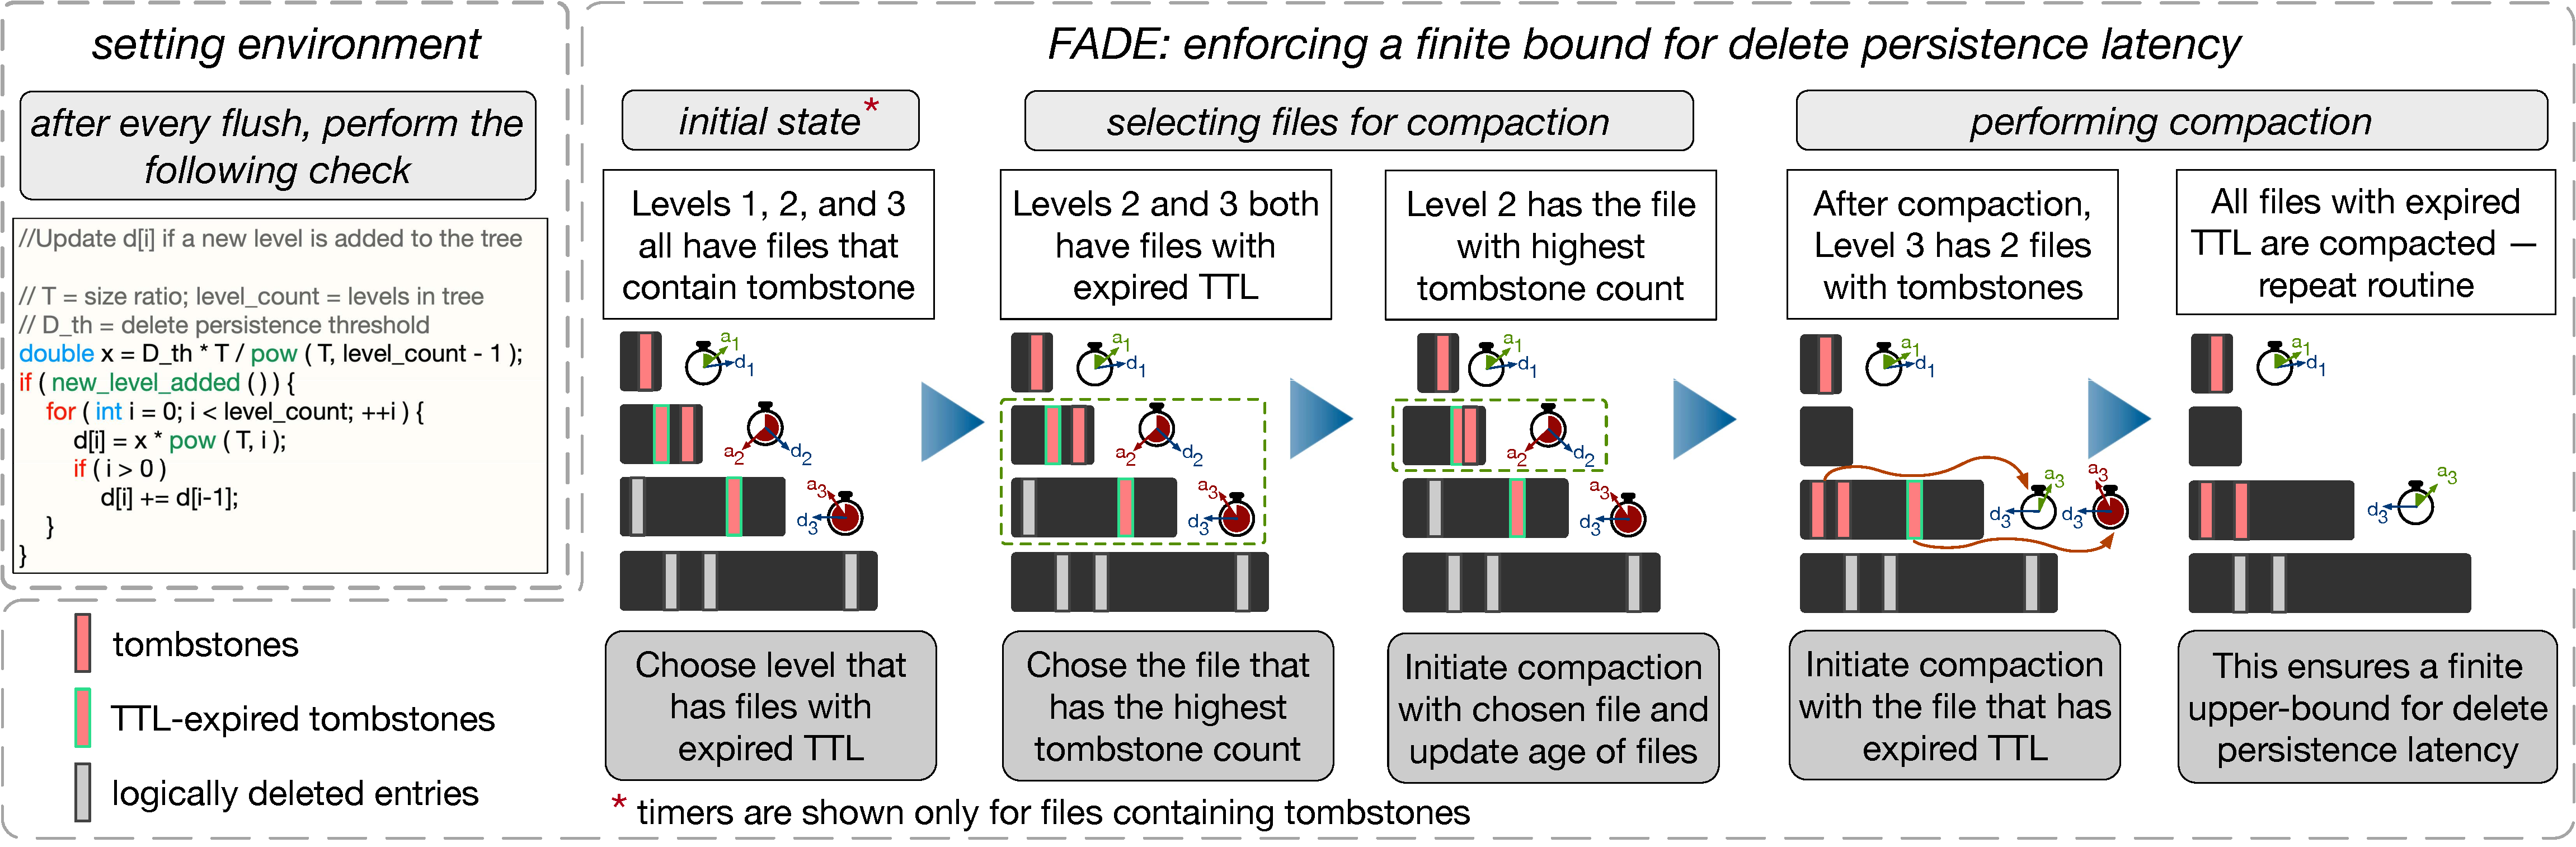
\includegraphics[width=\textwidth]{figs/effacingcompaction.pdf} 
        \vspace{-0.25in}        
    \caption{FADE persists tombstones within DPT, thus, improving overall performance.}
    \label{fig:ec} 
\vspace{0.2in}        
\end{figure} 

\begin{figure}[t]
    \centering  
        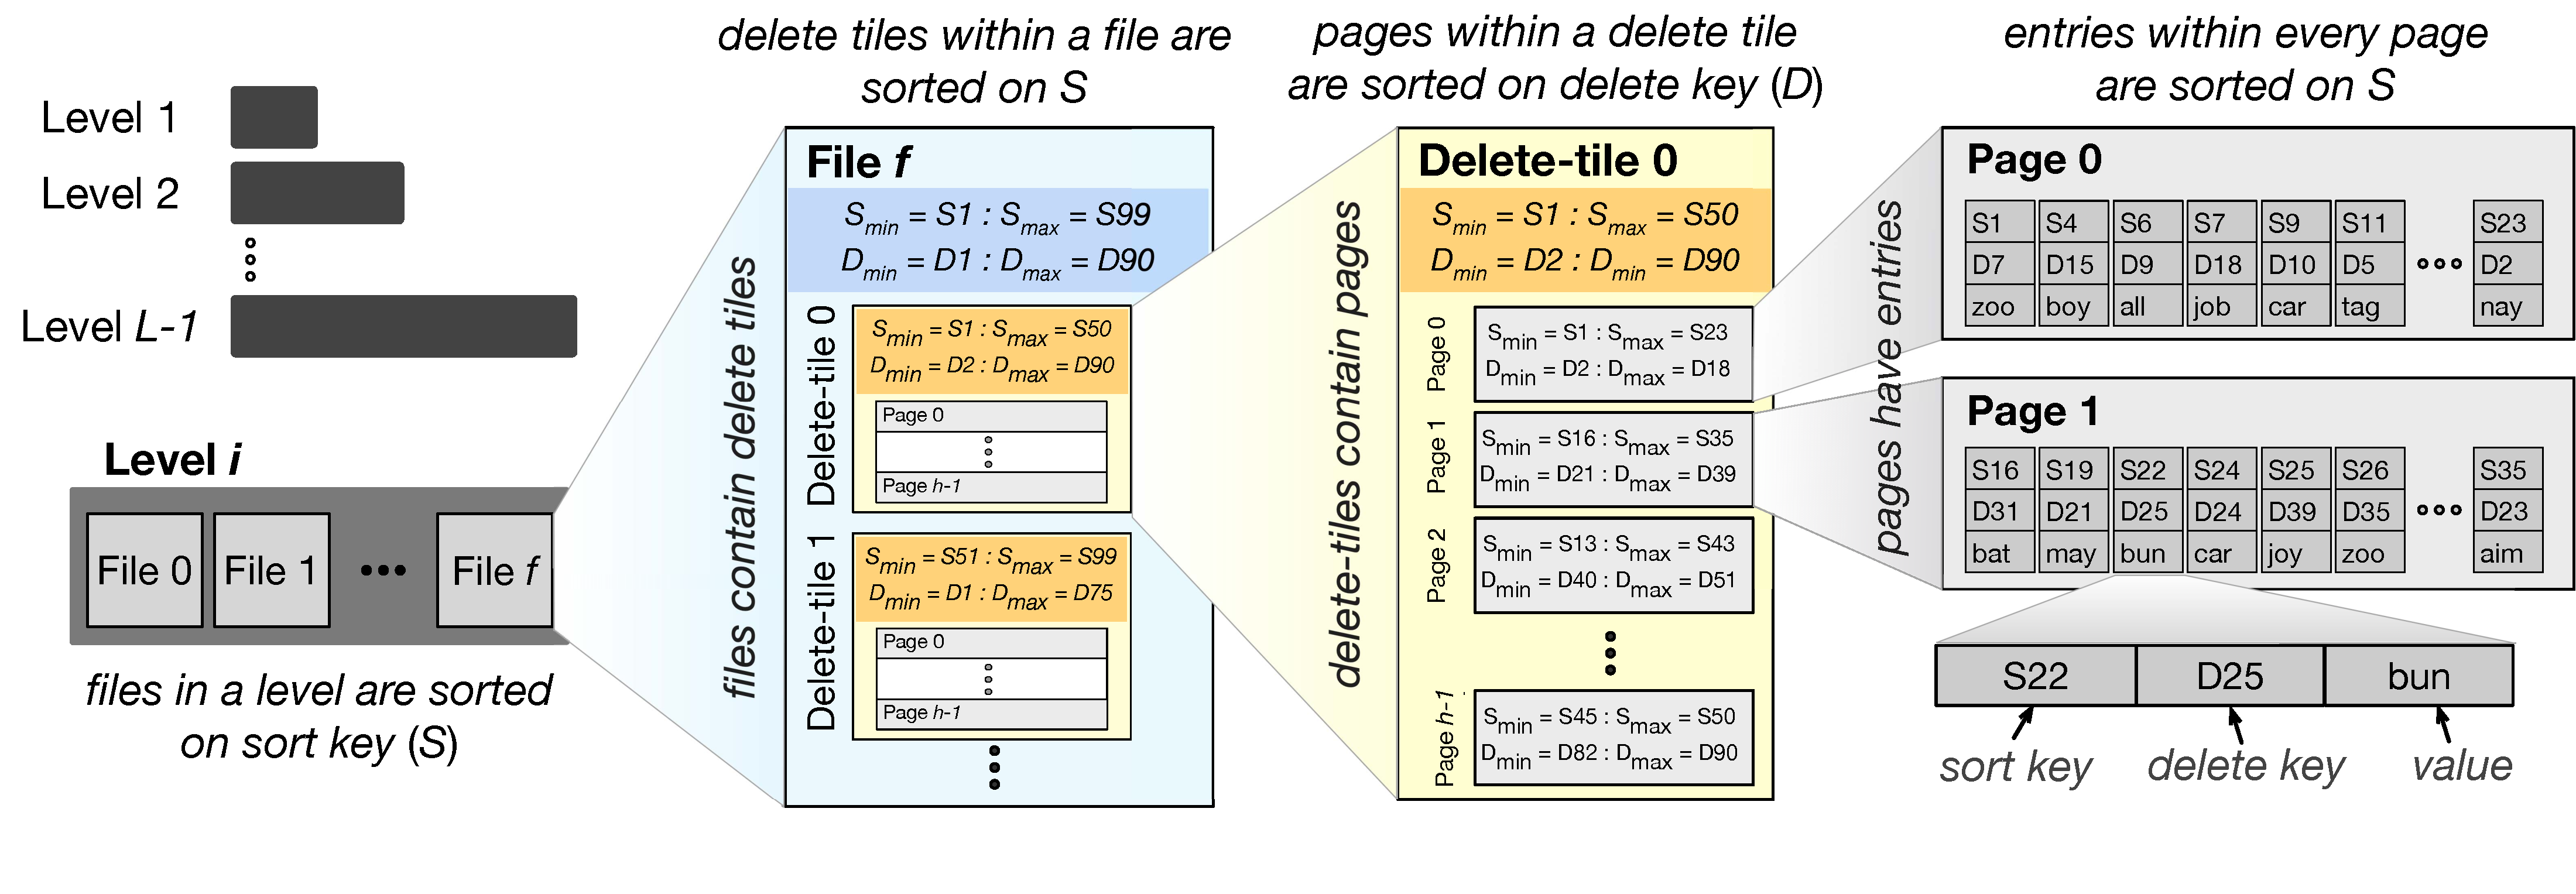
\includegraphics[width=\textwidth]{figs/storage_layout.pdf} 
   \vspace{-0.25in}        
    \caption{KiWi stores data in an interweaved fashion on the sort and delete key to facilitate efficient secondary range deletes while offering competitive  read performance.}
    \label{fig:layout} 
   \vspace{-0.15in}        
\end{figure} 


\Paragraph{Realizing Secondary Deletes}
As we discussed above, several instances of secondary deletes can be realized as
a collection of primary point deletes. However, when we are frequently tasked to
deleted a range of values based on a secondary attribute, we can achieve something
significantly better. In particular, a new weaved data layout between the original
sort key and the (secondary) delete key can offer much more efficient and timely
secondary range deletion while maintaining competitive read performance. The key idea is
to create a nested data organization that alternates between organizing data
based on the sort key (to facilitate good search performance) and based on the
delete key (to allow for consecutive chunks of data to be deleted at a time). 

This approach is implemented in the KiWi data layout~\cite{Sarkar2020} as shown in
Figure~\ref{fig:layout}. The core idea is that while the major components of the
database (files) are organized based on the sort key, every file is composed of
delete tiles that are internally organized based on the delete key,
partitioning the data accordingly. Lastly, each data page is again organized on
the search key to facilitate efficient in-memory search. The benefit for this
weaved data layout is that in the case of secondary range deletes, we can discard
entire groups of pages at a time, signaling the file system to reclaim this page
instantly, essentially converting the secondary delete to a page reclamation action
that has very low latency compared to a full database reorganization. In the 
worst case, we will have to in-place edit a few pages at the edge of the range, 
which is a tunable parameter that controls the maximum secondary deletion 
persistence latency as a tradeoff vs. read performance. 

\Paragraph{Evaluation} 
The approaches presented above for timely deletion were implemented as part of the
LSM-based system Lethe~\cite{Sarkar2020}, and achieved efficient timely
deletion respecting predetermined guarantees. The left hand-side of Figure~\ref{fig:results} shows the CDF of the 
tombstone age while varying the desired DPT to 16\%, 25\%, and 50\% of the duration
of the experiment. The colored areas correspond to the number of cumulative 
tombstones for the corresponding age on the x-axis, while the horizontal dotted-line
is the desired DPT. We observe that Lethe was able to always deliver the
requested DPT. The gray area corresponds to the age of tombstones of the state of
the art, where no DPT is imposed and deletes are not persisted timely. Notably, we also measured that enforcing the 
desired DPT shows benefits in terms of access time because the amount of invalid 
data was reduced. Similarly, we saw benefits in space amplification, and only marginal
cost increase in amortized write amplification.

The right hand-side of Figure~\ref{fig:results} shows the fraction of fully dropped
pages during a range delete as we vary the size of the delete tiles. We observe
that the fraction of pages fully dropped increases with the delete tile size, allowing
for efficient reclamation of the invalid data. Conversely, the read queries become
more expensive as we allow for more page drops, so the ideal delete tile size should
be tuned based on the workload. 


\begin{figure}[t]
    \centering  
        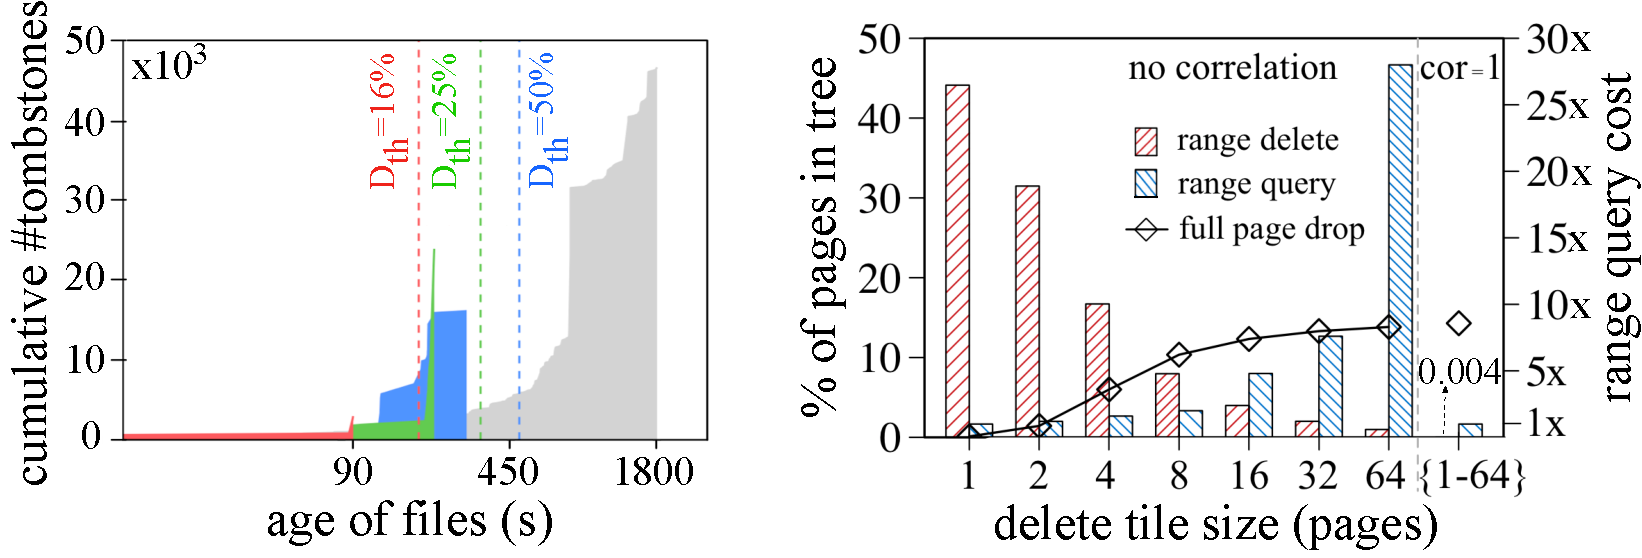
\includegraphics[width=\textwidth]{figs/lethe_figures.pdf} 
   \vspace{-0.25in}        
    \caption{Lethe ensures timely persistence of logically invalidated data within LSM-based out-of-place data systems for both primary and secondary classes of deletes.}
    \label{fig:results} 
   \vspace{-0.15in}        
\end{figure} 

\newpage
\Paragraph{Deletes in a Complex Data Model} The previous discussion focuses on
handling deletes in a per-instance manner without considering multiple copies of the
data in a more complex setting. Cohn-Gordon \textit{et al.}~\cite{Cohn-Gordon2020} proposed the deletion 
framework \textit{DELF} that ensures reliable data deletion from an online social 
network (OSN). 
\textit{DELF} enables detection of inconsistent data deletion in OSNs and also 
facilitates data recovery in cases where user data was incorrectly deleted. 
Minaei \textit{et al.}~\cite{Minaei2019} proposed a framework for persistently deleting all instances 
of user data in presence of observers, thereby, ensuring privacy through timely 
content concealment and removal. 





 
\section{Challenges and Opportunities}
\label{sec:challenges}
\vspace{-0.075in}



In Section~\ref{sec:vision}, we outlined the steps taken to realize the four-layered
vision of delete-compliant data systems presented in Figure~\ref{fig: vision}, 
however, there are still open questions and challenges for such systems which pose
opportunities for further innovative systems research.



\Paragraph{Device-level Deletion}
Data management solutions rely on storage devices and treat them as black boxes.
However, deleting data persistently at the device level and from data archives is an open 
technological challenge. Current endeavors in this direction are mainly focused on 
encryption-based solutions~\cite{Kissel2014,Koppel2013,Li2019a}.
Nevertheless, retention-based deletes entail persistent deletion of a ``quantum'' of data 
(e.g., the data ingested in a day) posing the following challenges for 
encryption-based solutions.
First, it is hard to \textit{determine the encryption granularity} while minimizing 
the encrypt/decrypt overhead. Second, with several data streams for different users/applications (and thus, bound by different SLAs), 
it is hard to \textit{manage the encryption keys efficiently and in a scalable manner}.
Third, efficient and scalable \textit{deletion from archives and backup stores on-demand} is hard to be supported by encryption-based deletion as the encrypt/decrypt cost and the fine encryption granularity adds prohibitive overheads.
Finally, from a legislation point-of-view it is not yet clear whether encrypting
and discarding the key is an accepted form of deletion.

When considering a system-level deletion similar approach to the one presented in 
Section~\ref{subsec:system-level} storage devices are essentially one more level of 
managing data at the physical layer and similar approaches have to be implemented
in the file system or the file and data systems have to be developed in tandem.

\Paragraph{Cloud-Level Deletion}
Further, operating on the cloud, data systems use virtualized devices and
object storage which is even more abstract hiding the details of how the 
low-level device and page management is taking place. Offering guarantees for
timely data deletion in virtualized storage will require a similar multi-layered
approach where the file system and the device firmware will expose knobs to allow
the application on top to request specific page reclamation properties. 





\Paragraph{Deletion in Distributed/Federated Computing Environment} 
With more and more data stores being transformed to cloud-based stores, user data 
may be collected, processed, and stored across multiple domains, spread across 
different geographic locations~\cite{Sarkar2018}. 
With different geographic locations being bound by different privacy regulations, we 
need to design \textit{solutions to ensure consistency for persistent deletion} of 
user data. 
Our intuition is that existing solutions for data stream-tainting~\cite{Enck2010}, 
cross-domain data tracing~\cite{Demsky2011,Herbster2016}, and related data 
provenance solutions~\cite{Buneman2018,Hasan2019} can be useful to address this 
problem.



\Paragraph{Compliance Demonstration} 
Last but certainly not least, data systems have to be able to prove compliance
when audited. The natural way to do so now is via log auditing, however, a more
light-weight algorithmic way for providing this will benefit both systems and users.
Inspecting logs and the underlying data is a time-consuming process and the 
long-term goal of the community should be to design system-level tools that can 
verifiably prove compliance with the privacy regulations. 
One interesting development in this direction is the evolution of security-driven 
operating systems, such as seL4~\cite{Klein2010,SeL4}. 
Another approach that can be taken is to show that the codebase of a data system
has the necessary code-paths for timely deletion via static and dynamic analysis.
An open challenge is to develop static and dynamic analysis tools that can prove
that a system deletes data respecting the timely deletion requirements set.









 
\section{Conclusion}
\label{sec:conclusion}
\vspace{-0.075in}

In this paper, we highlight that the recently enacted regulations  mandate
new data deletion requirements, requiring a new breed of data systems to support
them. We show that existing state-of-the-art out-of-place systems are ill-equipped
for this task, and we present a four-layered approach towards building the necessary
infrastructure. We present recent work on that front, and we conclude by discussing
several open research challenges.

\Paragraph{Acknowledgments} This work was partially funded by National
Science Foundation under Grant No. IIS-1850202 and a Facebook
Faculty Research Award.




 

\begin{thebibliography}{10}
\itemsep=1pt
\begin{small}


  \bibitem{UKGDPR}
  {Right to erasure}.
  \newblock {\em
    https://ico.org.uk/for-organisations/guide-to-data-protection/guide-to-the-general-data-protection-regulation-gdpr/individual-rights/right-to-erasure/}.
  
  \bibitem{GDPR}
  {Regulation (EU) 2016/679 of the European Parliament and of the council of 27
    April 2016 on the protection of natural persons with regard to the processing
    of personal data and on the free movement of such data, and repealing
    Directive 95/46/EC}.
  \newblock {\em Official Journal of the European Union (Legislative Acts)},
    pages L119/1 -- L119/88, 2016.
  
  \bibitem{CCPA2018}
  {California Consumer Privacy Act}.
  \newblock {\em Assembly Bill No. 375, Chapter 55}, 2018.
  
  \bibitem{DPA2018}
  {Data Protection Act 2018}.
  \newblock {\em
    https://www.legislation.gov.uk/ukpga/2018/12/pdfs/ukpga{\_}20180012{\_}en.pdf},
    2018.
  
  \bibitem{PIPEDA2019}
  {PIPEDA in brief}.
  \newblock {\em
    https://www.priv.gc.ca/en/privacy-topics/privacy-laws-in-canada/the-personal-information-protection-and-electronic-documents-act-pipeda/pipeda{\_}brief/},
    2019.
  
  \bibitem{CPRA}
  {The California Privacy Rights Act of 2020}.
  \newblock {\em https://thecpra.org/}, 2020.
  
  \bibitem{VCPDA}
  {Virginia Consumer Data Protection Act}.
  \newblock {\em
    https://www.sullcrom.com/files/upload/SC-Publication-Virginia-Second-State-Enact-Privacy-Legislation.pdf},
    2021.
  
  \bibitem{AmazonRedshift}
  Amazon.
  \newblock {Redshift}.
  \newblock {\em https://aws.amazon.com/redshift/}.
  
  \bibitem{Ambrose2013}
  M.~L. Ambrose and J.~Ausloos.
  \newblock {The Right to Be Forgotten Across the Pond}.
  \newblock {\em Journal of Information Policy}, 3:1--23, 2013.
  
  \bibitem{ApacheAccumulo}
  Apache.
  \newblock {Accumulo}.
  \newblock {\em https://accumulo.apache.org/}.
  
  \bibitem{ApacheHBase}
  Apache.
  \newblock {HBase}.
  \newblock {\em http://hbase.apache.org/}.
  
  \bibitem{ApacheCassandra}
  Apache.
  \newblock {Cassandra}.
  \newblock {\em http://cassandra.apache.org}, 2021.
  
  \bibitem{Athanassoulis2011}
  M.~Athanassoulis, S.~Chen, A.~Ailamaki, P.~B. Gibbons, and R.~Stoica.
  \newblock {MaSM: Efficient Online Updates in Data Warehouses}.
  \newblock In {\em Proceedings of the ACM SIGMOD International Conference on
    Management of Data}, pages 865--876, 2011.
  
  \bibitem{Athanassoulis2015}
  M.~Athanassoulis, S.~Chen, A.~Ailamaki, P.~B. Gibbons, and R.~Stoica.
  \newblock {Online Updates on Data Warehouses via Judicious Use of Solid-State
    Storage}.
  \newblock {\em ACM Transactions on Database Systems (TODS)}, 40(1), 2015.
  
  \bibitem{Athanassoulis2016}
  M.~Athanassoulis, M.~S. Kester, L.~M. Maas, R.~Stoica, S.~Idreos, A.~Ailamaki,
    and M.~Callaghan.
  \newblock {Designing Access Methods: The RUM Conjecture}.
  \newblock In {\em Proceedings of the International Conference on Extending
    Database Technology (EDBT)}, pages 461--466, 2016.
  
  \bibitem{Bender2000}
  M.~A. Bender, E.~D. Demaine, and M.~Farach-Colton.
  \newblock {Cache-Oblivious B-Trees}.
  \newblock In {\em Proceedings of the Annual Symposium on Foundations of
    Computer Science (FOCS)}, pages 399--409, 2000.
  
  \bibitem{Bender2015}
  M.~A. Bender, M.~Farach-Colton, W.~Jannen, R.~Johnson, B.~C. Kuszmaul, D.~E.
    Porter, J.~Yuan, and Y.~Zhan.
  \newblock {An Introduction to B$\epsilon$-trees and Write-Optimization}.
  \newblock {\em White Paper}, 2015.
  
  \bibitem{Brown2016}
  C.~T. Brown and T.~D. Manoranjan.
  \newblock {South Korea Releases Guidance on Right to Be Forgotten}.
  \newblock {\em
    https://www.lexology.com/library/detail.aspx?g=21be3837-0c43-4047-b8b5-9e863960b0b9},
    2016.
  
  \bibitem{Brown2021}
  G.~A. Brown.
  \newblock {Consumers' "Right to Delete" under US State Privacy Laws}.
  \newblock {\em
    https://www.securityprivacybytes.com/2021/03/consumers-right-to-delete-under-us-state-privacy-laws/},
    2021.
  
  \bibitem{Buneman2018}
  P.~Buneman and W.-C. Tan.
  \newblock {Data Provenance: What next?}
  \newblock {\em SIGMOD Rec.}, 47(3):5--16, 2018.
  
  \bibitem{Callaghan2020}
  M.~Callaghan.
  \newblock {Deletes are fast and slow in an LSM}.
  \newblock {\em
    http://smalldatum.blogspot.com/2020/01/deletes-are-fast-and-slow-in-lsm.html},
    2020.
  
  \bibitem{Cao2020}
  Z.~Cao, S.~Dong, S.~Vemuri, and D.~H.~C. Du.
  \newblock {Characterizing, Modeling, and Benchmarking RocksDB Key-Value
    Workloads at Facebook}.
  \newblock In {\em Proceedings of the USENIX Conference on File and Storage
    Technologies (FAST)}, pages 209--223, 2020.
  
  \bibitem{Carter2013}
  E.~L. Carter.
  \newblock {Argentina's Right to be Forgotten}.
  \newblock {\em Emory International Law Review}, 27(1), 2013.
  
  \bibitem{Chang2006}
  F.~Chang, J.~Dean, S.~Ghemawat, W.~C. Hsieh, D.~A. Wallach, M.~Burrows,
    T.~Chandra, A.~Fikes, and R.~E. Gruber.
  \newblock {Bigtable: A Distributed Storage System for Structured Data}.
  \newblock In {\em Proceedings of the USENIX Symposium on Operating Systems
    Design and Implementation (OSDI)}, pages 205--218, 2006.
  
  \bibitem{Chik2013}
  W.~B. Chik.
  \newblock {The Singapore Personal Data Protection Act and an assessment of
    future trends in data privacy reform}.
  \newblock {\em Comput. Law Secur. Rev.}, 29(5):554--575, 2013.
  
  \bibitem{Cisco2018}
  Cisco.
  \newblock {Cisco Global Cloud Index: Forecast and Methodology, 2016–2021}.
  \newblock {\em White Paper}, 2018.
  
  \bibitem{Cohn-Gordon2020}
  K.~Cohn-Gordon, G.~Damaskinos, D.~Neto, J.~Cordova, B.~Reitz, B.~Strahs,
    D.~Obenshain, P.~Pearce, I.~Papagiannis, and A.~Media.
  \newblock {DELF: Safeguarding deletion correctness in Online Social Networks}.
  \newblock In {\em 29th USENIX Security Symposium, USENIX Security 2020, August
    12-14, 2020}, 2020.
  
  \bibitem{Dageville2016}
  B.~Dageville, T.~Cruanes, M.~Zukowski, V.~Antonov, A.~Avanes, J.~Bock,
    J.~Claybaugh, D.~Engovatov, M.~Hentschel, J.~Huang, A.~W. Lee, A.~Motivala,
    A.~Q. Munir, S.~Pelley, P.~Povinec, G.~Rahn, S.~Triantafyllis, and
    P.~Unterbrunner.
  \newblock {The Snowflake Elastic Data Warehouse}.
  \newblock In {\em Proceedings of the ACM SIGMOD International Conference on
    Management of Data}, pages 215--226, 2016.
  
  \bibitem{Databricks}
  Databricks.
  \newblock {Online reference}.
  \newblock {\em https://databricks.com/}.
  
  \bibitem{Databricks2021}
  Databricks.
  \newblock {Table deletes, updates, and merges}.
  \newblock {\em
    https://docs.databricks.com/delta/delta-update.html{\#}delete-from-a-table},
    2021.
  
  \bibitem{Dayan2017}
  N.~Dayan, M.~Athanassoulis, and S.~Idreos.
  \newblock {Monkey: Optimal Navigable Key-Value Store}.
  \newblock In {\em Proceedings of the ACM SIGMOD International Conference on
    Management of Data}, pages 79--94, 2017.
  
  \bibitem{DeCandia2007}
  G.~DeCandia, D.~Hastorun, M.~Jampani, G.~Kakulapati, A.~Lakshman, A.~Pilchin,
    S.~Sivasubramanian, P.~Vosshall, and W.~Vogels.
  \newblock {Dynamo: Amazon's Highly Available Key-value Store}.
  \newblock {\em ACM SIGOPS Operating Systems Review}, 41(6):205--220, 2007.
  
  \bibitem{Demsky2011}
  B.~Demsky.
  \newblock {Cross-application data provenance and policy enforcement}.
  \newblock {\em ACM Transactions on Information Systems (TOIS)},
    14(1):6:1----6:22, 2011.
  
  \bibitem{Deng2020}
  F.~Deng, Q.~Cao, S.~Wang, S.~Liu, J.~Yao, Y.~Dong, and P.~Yang.
  \newblock {SeRW: Adaptively Separating Read and Write upon SSDs of Hybrid
    Storage Server in Clouds}.
  \newblock In {\em Proceedings of the International Conference on Parallel
    Processing (ICPP)}, pages 76:1----76:11, 2020.
  
  \bibitem{Deshpande2018}
  A.~Deshpande and A.~Machanavajjhala.
  \newblock {ACM SIGMOD Blog: Privacy Challenges in the Post-GDPR World: A Data
    Management Perspective}.
  \newblock {\em http://wp.sigmod.org/?p=2554}, 2018.
  
  \bibitem{Dong2017}
  S.~Dong, M.~Callaghan, L.~Galanis, D.~Borthakur, T.~Savor, and M.~Strum.
  \newblock {Optimizing Space Amplification in RocksDB}.
  \newblock In {\em Proceedings of the Biennial Conference on Innovative Data
    Systems Research (CIDR)}, 2017.
  
  \bibitem{Enck2010}
  W.~Enck, P.~Gilbert, B.-G. Chun, L.~P. Cox, J.~Jung, P.~D. McDaniel, and
    A.~Sheth.
  \newblock {TaintDroid: An Information-Flow Tracking System for Realtime Privacy
    Monitoring on Smartphones}.
  \newblock In {\em Proceedings of the USENIX Symposium on Operating Systems
    Design and Implementation (OSDI)}, pages 393--407, 2010.
  
  \bibitem{FacebookRocksDB}
  Facebook.
  \newblock {RocksDB}.
  \newblock {\em https://github.com/facebook/rocksdb}, 2021.
  
  \bibitem{Farber2012}
  F.~F{\"{a}}rber, N.~May, W.~Lehner, P.~Gro{\ss}e, I.~M{\"{u}}ller, H.~Rauhe,
    and J.~Dees.
  \newblock {The SAP HANA Database -- An Architecture Overview}.
  \newblock {\em IEEE Data Engineering Bulletin}, 35(1):28--33, 2012.
  
  \bibitem{Gartner2017}
  Gartner.
  \newblock {Gartner Says 8.4 Billion Connected ``Things" Will Be in Use in 2017,
    Up 31 Percent From 2016}.
  \newblock https://tinyurl.com/Gartner2020, 2017.
  
  \bibitem{Goddard2017}
  M.~Goddard.
  \newblock {The EU General Data Protection Regulation (GDPR): European
    Regulation that has a Global Impact}.
  \newblock {\em International Journal of Market Research}, 59(6):703--705, 2017.
  
  \bibitem{Golan-Gueta2015}
  G.~Golan-Gueta, E.~Bortnikov, E.~Hillel, and I.~Keidar.
  \newblock {Scaling Concurrent Log-Structured Data Stores}.
  \newblock In {\em Proceedings of the ACM European Conference on Computer
    Systems (EuroSys)}, pages 32:1--32:14, 2015.
  
  \bibitem{GoogleLevelDB}
  Google.
  \newblock {LevelDB}.
  \newblock {\em https://github.com/google/leveldb/}, 2021.
  
  \bibitem{Gupta2015}
  A.~Gupta, D.~Agarwal, D.~Tan, J.~Kulesza, R.~Pathak, S.~Stefani, and
    V.~Srinivasan.
  \newblock {Amazon Redshift and the Case for Simpler Data Warehouses}.
  \newblock In {\em Proceedings of the ACM SIGMOD International Conference on
    Management of Data}, pages 1917--1923, 2015.
  
  \bibitem{Hasan2019}
  S.~S. Hasan, N.~H. Sultan, and F.~A. Barbhuiya.
  \newblock {Cloud Data Provenance using IPFS and Blockchain Technology}.
  \newblock In {\em Proceedings of the International Workshop on Security in
    Cloud Computing (SCC)}, pages 5--12, 2019.
  
  \bibitem{Heman2010}
  S.~H{\'{e}}man, M.~Zukowski, and N.~J. Nes.
  \newblock {Positional Update Handling in Column Stores}.
  \newblock In {\em Proceedings of the ACM SIGMOD International Conference on
    Management of Data}, pages 543--554, 2010.
  
  \newpage
  \bibitem{Herbster2016}
  R.~Herbster, S.~DellaTorre, P.~Druschel, and B.~Bhattacharjee.
  \newblock {Privacy Capsules: Preventing Information Leaks by Mobile Apps}.
  \newblock In {\em Proceedings of the 14th Annual International Conference on
    Mobile Systems, Applications, and Services, MobiSys 2016, Singapore, June
    26-30, 2016}, pages 399--411, 2016.
  
  \bibitem{Huang2019}
  G.~Huang, X.~Cheng, J.~Wang, Y.~Wang, D.~He, T.~Zhang, F.~Li, S.~Wang, W.~Cao,
    and Q.~Li.
  \newblock {X-Engine: An Optimized Storage Engine for Large-scale E-commerce
    Transaction Processing}.
  \newblock In {\em Proceedings of the ACM SIGMOD International Conference on
    Management of Data}, pages 651--665, 2019.
  
  \bibitem{Idreos2019}
  S.~Idreos, N.~Dayan, W.~Qin, M.~Akmanalp, S.~Hilgard, A.~Ross, J.~Lennon,
    V.~Jain, H.~Gupta, D.~Li, and Z.~Zhu.
  \newblock {Design Continuums and the Path Toward Self-Designing Key-Value
    Stores that Know and Learn}.
  \newblock In {\em Proceedings of the Biennial Conference on Innovative Data
    Systems Research (CIDR)}, 2019.
  
  \bibitem{Idreos2012}
  S.~Idreos, F.~Groffen, N.~Nes, S.~Manegold, K.~S. Mullender, and M.~L. Kersten.
  \newblock {MonetDB: Two Decades of Research in Column-oriented Database
    Architectures}.
  \newblock {\em IEEE Data Engineering Bulletin}, 35(1):40--45, 2012.
  
  \bibitem{Jannen2015}
  W.~Jannen, J.~Yuan, Y.~Zhan, A.~Akshintala, J.~Esmet, Y.~Jiao, A.~Mittal,
    P.~Pandey, P.~Reddy, L.~Walsh, M.~A. Bender, M.~Farach-Colton, R.~Johnson,
    B.~C. Kuszmaul, and D.~E. Porter.
  \newblock {BetrFS: A Right-optimized Write-optimized File System}.
  \newblock In {\em Proceedings of the USENIX Conference on File and Storage
    Technologies (FAST)}, pages 301--315, 2015.
  
  \bibitem{Jones2012}
  M.~L. Jones.
  \newblock {It's About Time: Privacy, Information Lifecycles, and the Right to
    Be Forgotten}.
  \newblock {\em Stanford Technology Law Review}, 16(2):54, 2012.
  
  \bibitem{Kang2016}
  W.-H. Kang, S.-W. Lee, and B.~Moon.
  \newblock {Flash as cache extension for online transactional workloads}.
  \newblock {\em The VLDB Journal}, 25(5):673--694, 2016.
  
  \bibitem{Kissel2014}
  R.~Kissel, A.~Regenscheid, M.~Scholl, and K.~Stine.
  \newblock {Guidelines for Media Sanitization}.
  \newblock {\em NIST Special Publication 800-88}, 2014.
  
  \bibitem{Kittane2021}
  P.~Kittane, I.~S. Charles, A.~Kamath, and G.~Gokhale.
  \newblock {Privacy and Data Protection -- India Wrap 2020}.
  \newblock {\em The National Law Review}, XI(162), 2021.
  
  \bibitem{Klein2010}
  G.~Klein, J.~Andronick, K.~Elphinstone, G.~Heiser, D.~Cock, P.~Derrin,
    D.~Elkaduwe, K.~Engelhardt, R.~Kolanski, M.~Norrish, T.~Sewell, H.~Tuch, and
    S.~Winwood.
  \newblock {seL4: formal verification of an operating-system kernel}.
  \newblock {\em Communications of the ACM}, 53(6):107--115, 2010.
  
  \bibitem{Koppel2013}
  B.~K{\"{o}}ppel and S.~Neuhaus.
  \newblock {Analysis of a hardware security module's high-availability setting}.
  \newblock {\em IEEE Security Privacy}, 11(3):77--80, 2013.
  
  \bibitem{Kuszmaul2014}
  B.~C. Kuszmaul.
  \newblock {A Comparison of Fractal Trees to Log-Structured Merge (LSM) Trees}.
  \newblock {\em Tokutek White Paper}, 2014.
  
  \bibitem{Lamb2012}
  A.~Lamb, M.~Fuller, and R.~Varadarajan.
  \newblock {The Vertica Analytic Database: C-Store 7 Years Later}.
  \newblock {\em Proceedings of the VLDB Endowment}, 5(12):1790--1801, 2012.
  
  \bibitem{Li2019a}
  B.~Li and D.~H.~C. Du.
  \newblock {TASecure: Temperature-Aware Secure Deletion Scheme for Solid State
    Drives}.
  \newblock In {\em Proceedings of the Great Lakes Symposium on VLSI (GLSVLSI)},
    pages 275--278, 2019.
  
  \bibitem{LinkedInVoldemort}
  LinkedIn.
  \newblock {Voldemort}.
  \newblock {\em http://www.project-voldemort.com}.
  
  \bibitem{Luo2020b}
  C.~Luo and M.~J. Carey.
  \newblock {LSM-based Storage Techniques: A Survey}.
  \newblock {\em The VLDB Journal}, 29(1):393--418, 2020.
  
  \bibitem{Madan2018}
  A.~Madan and A.~Kryczka.
  \newblock {DeleteRange: A New Native RocksDB Operation}.
  \newblock {\em https://rocksdb.org/blog/2018/11/21/delete-range.html}, 2018.
  
  \bibitem{Piper2022}
  R.~McKean, E.~Kurowska-Tober, and H.~Waem.
  \newblock {DLA Piper GDPR fines and data breach survey: January 2022}.
  \newblock {\em
    https://www.dlapiper.com/en/us/insights/publications/2022/1/dla-piper-gdpr-fines-and-data-breach-survey-2022/},
    2022.
  
  \bibitem{Minaei2019}
  M.~Minaei, M.~Mondal, P.~Loiseau, K.~P. Gummadi, and A.~Kate.
  \newblock {Lethe: Conceal Content Deletion from Persistent Observers}.
  \newblock {\em Proceedings on Privacy Enhancing Technologies (PoPET)},
    2019(1):206--226, 2019.
  
  \bibitem{ONeil1996}
  P.~E. O'Neil, E.~Cheng, D.~Gawlick, and E.~J. O'Neil.
  \newblock {The log-structured merge-tree (LSM-tree)}.
  \newblock {\em Acta Informatica}, 33(4):351--385, 1996.
  
  \bibitem{Papadopoulos2016}
  S.~Papadopoulos, K.~Datta, S.~Madden, and T.~Mattson.
  \newblock {The TileDB Array Data Storage Manager}.
  \newblock {\em Proceedings of the VLDB Endowment}, 10(4):349--360, 2016.
  
  \bibitem{Paradigm4}
  Paradigm4.
  \newblock {Online reference}.
  \newblock {\em https://www.paradigm4.com/}.
  
  \bibitem{Pardo2020}
  D.~Pardo.
  \newblock {First Decision on the "Right to be Forgotten" in Argentina}.
  \newblock {\em
    https://scholarlycommons.law.emory.edu/cgi/viewcontent.cgi?article=1097{\&}context=eilr},
    2020.
  
  \bibitem{DLAPiper2020}
  D.~Piper.
  \newblock {GDPR Data Breach Survey 2020}.
  \newblock {\em
    https://www.dlapiper.com/en/us/insights/publications/2020/01/gdpr-data-breach-survey-2020/},
    2020.
  
  \bibitem{Sadoghi2016}
  M.~Sadoghi, K.~A. Ross, M.~Canim, and B.~Bhattacharjee.
  \newblock {Exploiting SSDs in operational multiversion databases}.
  \newblock {\em The VLDB Journal}, 25(5):651--672, 2016.
  
  \bibitem{Sarkar2022a}
  S.~Sarkar, K.~Chen, Z.~Zhu, and M.~Athanassoulis.
  \newblock {Compactionary: A Dictionary for LSM Compactions}.
  \newblock In {\em Proceedings of the ACM SIGMOD International Conference on
    Management of Data}, 2022.
  
  \bibitem{Sarkar2022b}
  S.~Sarkar and M.~Athanassoulis.
  \newblock {Dissecting, Designing, and Optimizing LSM-based Data Stores}.
  \newblock In {\em Proceedings of the ACM SIGMOD International Conference on
    Management of Data}, 2022.
  
  \bibitem{Sarkar2022}
  S.~Sarkar and M.~Athanassoulis.
  \newblock {Query Language Support for Timely Data Deletion}.
  \newblock In {\em Proceedings of the International Conference on Extending
    Database Technology (EDBT)}, 2022.
  
  \bibitem{Sarkar2018}
  S.~Sarkar, J.-P. Ban{\^{a}}tre, L.~Rilling, and C.~Morin.
  \newblock {Towards Enforcement of the EU GDPR: Enabling Data Erasure}.
  \newblock In {\em Proceedings of the IEEE International Conference of Internet
    of Things (iThings)}, pages 1--8, 2018.
  
  \bibitem{Sarkar2020}
  S.~Sarkar, T.~I. Papon, D.~Staratzis, and M.~Athanassoulis.
  \newblock {Lethe: A Tunable Delete-Aware LSM Engine}.
  \newblock In {\em Proceedings of the ACM SIGMOD International Conference on
    Management of Data}, pages 893--908, 2020.
  
  \bibitem{Sarkar2021c}
  S.~Sarkar, D.~Staratzis, Z.~Zhu, and M.~Athanassoulis.
  \newblock {Constructing and Analyzing the LSM Compaction Design Space}.
  \newblock {\em Proceedings of the VLDB Endowment}, 14(11):2216--2229, 2021.
  
  \bibitem{Schwarzkopf2019}
  M.~Schwarzkopf, E.~Kohler, M.~F. Kaashoek, and R.~T. Morris.
  \newblock {Position: GDPR Compliance by Construction}.
  \newblock In {\em Selected Papers from VLDB Workshop on Polystore Systems for
    Heterogeneous Data in Multiple Databases with Privacy and Security Assurances
    (POLY)}, volume 11721 of {\em Lecture Notes in Computer Science}, pages
    39--53, 2019.
  
  \bibitem{Sears2012}
  R.~Sears and R.~Ramakrishnan.
  \newblock {bLSM: A General Purpose Log Structured Merge Tree}.
  \newblock In {\em Proceedings of the ACM SIGMOD International Conference on
    Management of Data}, pages 217--228, 2012.
  
  \bibitem{SeL4}
  SeL4.
  \newblock {Online reference}.
  \newblock {\em https://sel4.systems}.
  
  \bibitem{Shah2019}
  A.~Shah, V.~Banakar, S.~Shastri, M.~Wasserman, and V.~Chidambaram.
  \newblock {Analyzing the Impact of GDPR on Storage Systems}.
  \newblock In {\em Proceedings of the USENIX Conference on Hot Topics in Storage
    and File Systems (HotStorage)}, 2019.
  
  \bibitem{Shastri2020}
  S.~Shastri, V.~Banakar, M.~Wasserman, A.~Kumar, and V.~Chidambaram.
  \newblock {Understanding and Benchmarking the Impact of GDPR on Database
    Systems}.
  \newblock {\em Proceedings of the VLDB Endowment}, 13(7):1064--1077, 2020.
  
  \bibitem{Shastri2019}
  S.~Shastri, M.~Wasserman, and V.~Chidambaram.
  \newblock {The Seven Sins of Personal-Data Processing Systems under GDPR}.
  \newblock In {\em Proceedings of USENIX Workshop on Hot Topics in Cloud
    Computing (HotCloud)}, 2019.
  
  \bibitem{Shastri2021}
  S.~Shastri, M.~Wasserman, and V.~Chidambaram.
  \newblock {GDPR anti-patterns}.
  \newblock {\em Communications of the ACM}, 64(2):59--65, 2021.
  
  \bibitem{Stonebraker2005}
  M.~Stonebraker, D.~J. Abadi, A.~Batkin, X.~Chen, M.~Cherniack, M.~Ferreira,
    E.~Lau, A.~Lin, S.~R. Madden, E.~J. O'Neil, P.~E. O'Neil, A.~Rasin, N.~Tran,
    and S.~Zdonik.
  \newblock {C-Store: A Column-oriented DBMS}.
  \newblock In {\em Proceedings of the International Conference on Very Large
    Data Bases (VLDB)}, pages 553--564, 2005.
  
  \bibitem{Stonebraker2013}
  M.~Stonebraker, J.~Duggan, L.~Battle, and O.~Papaemmanouil.
  \newblock {SciDB DBMS Research at M.I.T}.
  \newblock {\em IEEE Data Eng. Bull.}, 36(4):21--30, 2013.
  
  \bibitem{Tessian2022}
  Tessian.
  \newblock {25 Biggest GDPR Fines So Far (2019, 2020, 2021, 2022)}.
  \newblock {\em https://www.tessian.com/blog/biggest-gdpr-fines-2020/}, 2022.
  
  \bibitem{TileDB}
  TileDB.
  \newblock {Online reference}.
  \newblock {\em https://tiledb.io}.
  
  \bibitem{Tsesis2014}
  A.~Tsesis.
  \newblock {The Right to be Forgotten and Erasure: Privacy, Data Brokers, and
    the Indefinite Retention of Data}.
  \newblock {\em Wake Forest Law Review}, 48:51, 2014.
  
  \bibitem{Whittaker2019}
  Z.~Whittaker and N.~Lomas.
  \newblock {Even years later, Twitter doesn't delete your direct messages}.
  \newblock {\em https://techcrunch.com/2019/02/15/twitter-direct-messages/},
    2019.
  
  \bibitem{Yang2020}
  L.~Yang, H.~Wu, T.~Zhang, X.~Cheng, F.~Li, L.~Zou, Y.~Wang, R.~Chen, J.~Wang,
    and G.~Huang.
  \newblock {Leaper: A Learned Prefetcher for Cache Invalidation in LSM-tree
    based Storage Engines}.
  \newblock {\em Proceedings of the VLDB Endowment}, 13(11):1976--1989, 2020.
  
  \bibitem{Zheng2018}
  Q.~Zheng, C.~D. Cranor, D.~Guo, G.~R. Ganger, G.~Amvrosiadis, G.~A. Gibson,
    B.~W. Settlemyer, G.~Grider, and F.~Guo.
  \newblock {Scaling Embedded In-Situ Indexing with DeltaFS}.
  \newblock In {\em Proceedings of the ACM/IEEE International Conference for High
    Performance Computing, Networking, Storage and Analysis (SC)}, pages
    3:1--3:15, 2018.

\end{small}
\end{thebibliography}


\end{document}
